\section*{Chapter 3: Design and Implementation}
\phantomsection \label{chap:design} \setcounter{section}{3} \setcounter{subsection}{0}
\addcontentsline{toc}{section}{\textit{Chapter 3: Design and Implementation}}

The central question driving the design of \texttt{linux-mcp} is not how to make the gateway more robust, but which state the gateway should not be solely responsible for holding.
\texttt{mcpd} retains everything requiring semantic flexibility; \texttt{kernel\_\allowbreak mcp} owns the state that must survive gateway failure and remain unreachable by unprivileged processes.



\subsection{Design Goals}
\label{sec:design-goals}

The design is oriented around three concerns that arise from the problem of mediating LLM tool invocations in a trustworthy manner.

The foremost requirement is that admission control must not reduce to a user-space daemon unilaterally deciding whether to forward a request.
The admissibility of a tool invocation is determined solely by explicit kernel-resident state: the registration status of the requesting agent, the presence of the target tool in the registry, and the consistency of its semantic identity with the registered manifest.
Anchoring this decision in the kernel ensures it cannot be silently circumvented by tampering with the daemon or by injecting a forged request that the daemon would otherwise accept~\cite{chen2016shreds, brimhall2023mac}.

At the same time, the system must remain compatible with ordinary user-space tools.
Requiring tool authors to write against a kernel-facing API would break compatibility with existing tool ecosystems and make incremental deployment impractical.
Tool services therefore carry no kernel-facing obligations; the protocol they implement is described in Section~\ref{sec:wire-protocols}.

Another concern is observability.
Admission, approval, and completion events must not be confined to transient entries in a daemon's in-memory state or application-level logs. They must be queryable through the kernel's own interfaces, independently of whether \texttt{mcpd} is currently running.
This property is particularly relevant in the context of daemon failure: if \texttt{mcpd} crashes, the kernel-held state must remain inspectable without relying on any daemon-side representation.

These goals impose an explicit scope boundary on the design.
\texttt{linux-mcp} does not attempt to verify tool semantics at runtime, enforce a general policy language, or address every attack surface in LLM-based systems.
What it changes is specifically where admission decisions are made and where approval state is maintained.
The threat model grounding this scope is given in Chapter~\ref{chap:background}, Section~``Threat Model'', and is referenced throughout the mechanism descriptions that follow.



\subsection{System Architecture}
\label{sec:system-architecture}

\begin{figure}[t]
\centering
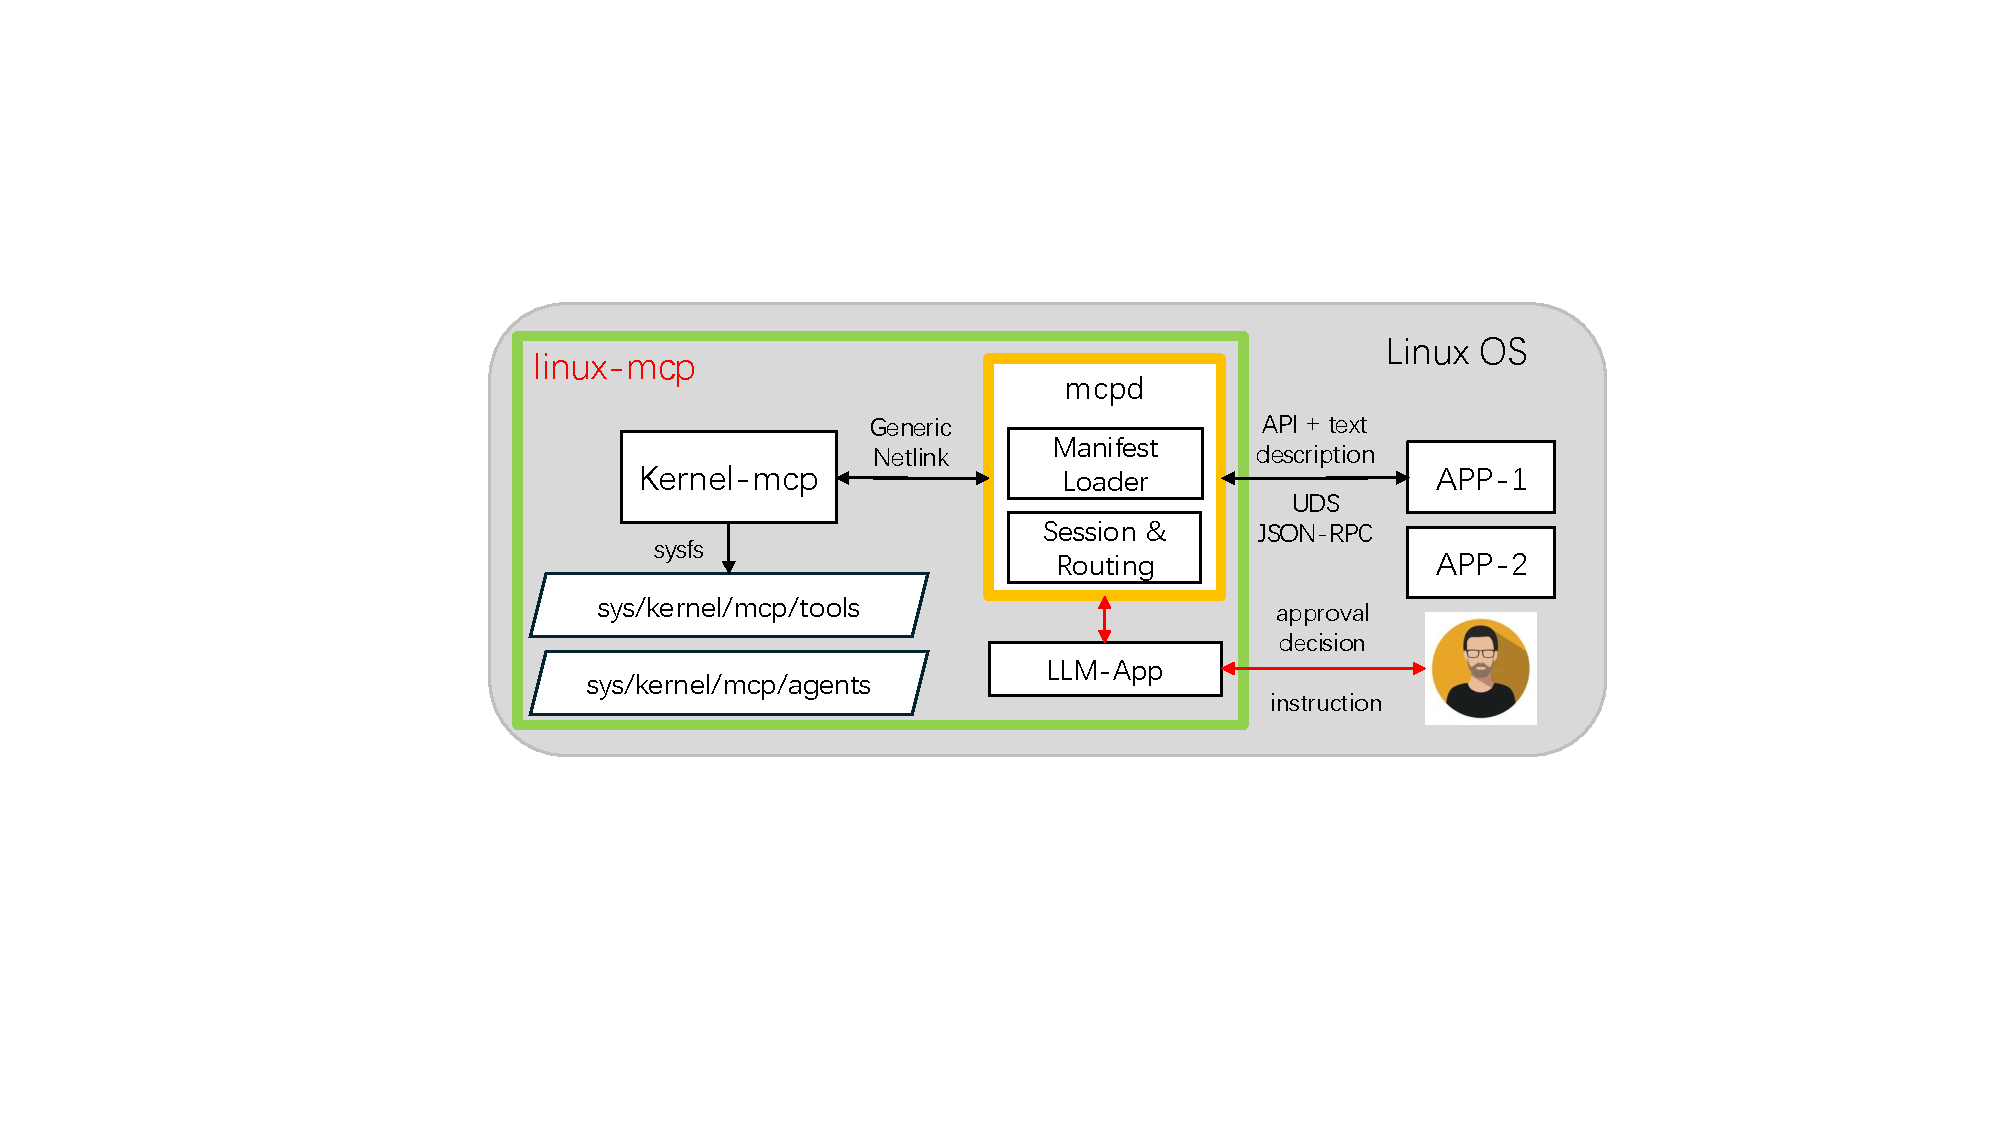
\includegraphics[width=\linewidth,trim=8cm 6cm 6.4cm 4.5cm,clip]{figures/linux-mcp-overview.pdf}
\caption{Overall architecture of \texttt{linux-mcp}.}
\label{fig:linux-mcp-overview}
\end{figure}

The overall architecture of \texttt{linux-mcp}, shown in Figure~\ref{fig:linux-mcp-overview}, comprises four components.

\texttt{llm-app} is the user-facing client.
It queries \texttt{mcpd} for the tool catalog, constructs invocation payloads from tool schemas, and submits requests.
The client has no direct interaction with the kernel module; all control-plane operations are mediated through \texttt{mcpd}.

\texttt{mcpd} is the user-space gateway and the semantic front-end of the control plane.
It is responsible for loading and validating tool manifests, computing manifest-derived semantic hashes, managing sessions, exposing catalog APIs (\texttt{list\_apps}, \texttt{list\_\allowbreak tools}), communicating with the kernel over Generic Netlink, and forwarding admitted requests to tool services over Unix domain sockets (UDS).
\texttt{mcpd} is the only component that sees both tool semantics and runtime endpoints, so it is the only one that needs changing when manifests or endpoints are reconfigured.

\texttt{kernel\_\allowbreak mcp} is a loadable kernel module implementing the \texttt{KERNEL\_\allowbreak MCP} Generic Netlink family.
It maintains the tool and agent registries, arbitrates invocation requests, manages approval ticket lifecycles, and exports per-tool and per-agent state through \texttt{sysfs} under \texttt{/\allowbreak sys/\allowbreak kernel/\allowbreak mcp/}.
It does not parse manifests, execute tools, or implement a policy language. Its only job is enforcing the admission-control invariants.

\texttt{tool-app} is the execution side: a collection of resident user-space services, each bound to a Unix domain socket.
When a request is admitted, \texttt{mcpd} forwards the payload to the appropriate tool service, which executes in an ordinary user-space environment and returns its result to \texttt{mcpd}, which then reports completion back to the kernel.

To clarify the separation of responsibilities across layers, Table~\ref{tab:architecture_layers} summarises each component together with its intended scope and explicitly excluded functionality.

\begin{table}[htbp]
\centering
\small
\begin{spacing}{1.1}
\begin{tabular}{l p{3cm} p{4.8cm} p{4.5cm}}
\toprule
\textbf{Layer} & \textbf{Component} & \textbf{Main responsibility} & \textbf{Intentionally excluded} \\
\midrule

Client layer
& \texttt{llm-app} CLI/GUI
& Discover tools, plan usage, open sessions, submit requests, handle approvals
& Direct tool access, direct kernel communication \\

Gateway layer
& \texttt{mcpd}
& Load manifests, compute semantic hash, validate payloads, bind sessions, route requests, communicate with kernel
& Durable governance state independent of process lifetime \\

Kernel layer
& \texttt{kernel\_\allowbreak mcp}
& Maintain registries, perform admission decisions, manage approval tickets, expose \texttt{sysfs} state
& JSON parsing, tool execution, LLM-specific logic \\

Execution layer
& Tool services
& Execute application logic and return structured results
& Global policy enforcement \\

\bottomrule
\end{tabular}
\end{spacing}
\caption{Concrete layers in \texttt{linux-mcp}.}
\label{tab:architecture_layers}
\end{table}



\subsection{Control-Plane Workflow}

\begin{figure}[t]
\centering
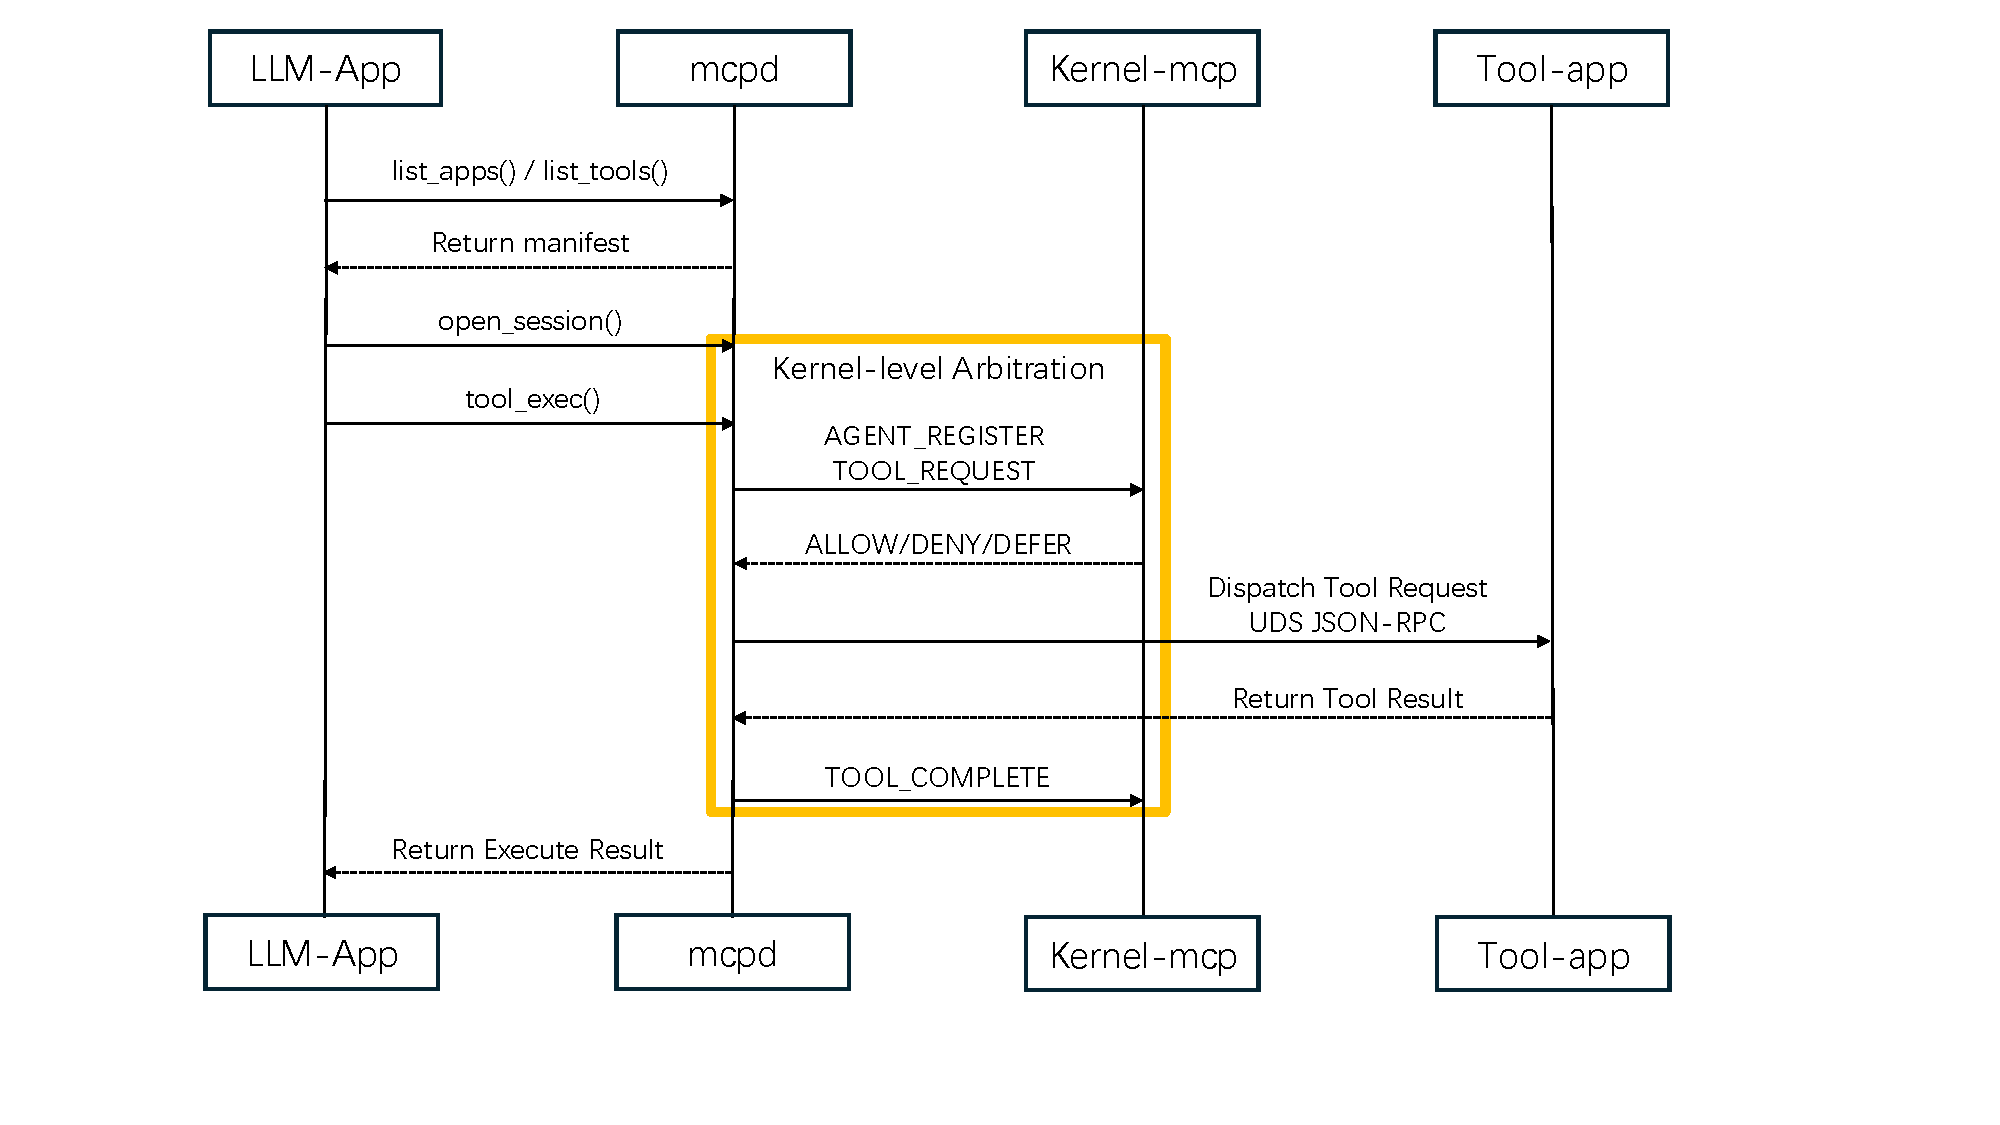
\includegraphics[width=\linewidth,trim=1cm 1.5cm 2cm 0cm,clip]{figures/linux-mcp-workload.pdf}
\caption{Invocation lifecycle in \texttt{linux-mcp}.}
\label{fig:chapter3-lifecycle}
\end{figure}

The end-to-end request path is:
\[
\texttt{llm-app} \to \texttt{mcpd} \to \texttt{kernel\_\allowbreak mcp} \to
\texttt{mcpd} \to \texttt{tool-app} \to \texttt{mcpd} \to \texttt{llm-app}
\]
Figure~\ref{fig:chapter3-lifecycle} illustrates this path as a sequence diagram.
A request originates in \texttt{llm-app}, which first issues a catalog query that \texttt{mcpd} satisfies from its manifest-derived in-memory state.
The kernel occupies this path not as a passive observer but as the active arbitration point: \texttt{mcpd} cannot forward a request to a tool without first obtaining an \texttt{ALLOW} decision from the kernel, and it cannot close an invocation without reporting \texttt{TOOL\_\allowbreak COMPLETE} back through the same channel.
Admission and completion are explicit, kernel-visible state transitions; the daemon no longer makes these decisions in private.

The client uses the catalog response to construct a structured invocation payload and submits it as a \texttt{tool:exec} call to \texttt{mcpd} (see Table~\ref{tab:llm-mcpd} for the message format).

Upon receiving the request, \texttt{mcpd} performs a series of user-space checks: it resolves the active session, validates the payload against the declared input schema, identifies the target tool, and retrieves the semantic hash associated with that tool from its manifest-derived state.
Only upon successful completion of these checks does \texttt{mcpd} issue a \texttt{TOOL\_\allowbreak REQUEST} to the kernel, supplying the agent identifier, tool identifier, and semantic hash as parameters.

The kernel module then performs arbitration.
It verifies that the requesting agent appears in the agent registry, that the target tool appears in the tool registry, and that the semantic hash in the request matches the hash recorded at registration time.
Based on these checks and the tool's declared policy, the kernel returns a decision that determines whether the request may proceed immediately, must be rejected outright, or requires external approval before execution.
The detailed semantics of these decisions are described in Figure~\ref{fig:chapter3-approval}.

Depending on the kernel's decision, \texttt{mcpd} either forwards the request to the tool service, terminates the invocation with an error, or transitions the request into a pending state awaiting explicit approval.
After the tool service returns a result, \texttt{mcpd} issues \texttt{TOOL\_\allowbreak COMPLETE} to the kernel, closing the invocation lifecycle from the control plane's perspective.

This workflow has a concrete security consequence: the kernel both opens and closes every invocation.
An invocation that never reaches \texttt{TOOL\_\allowbreak COMPLETE}, whether due to daemon failure or tool timeout, persists as an open entry in kernel state and remains inspectable via \texttt{sysfs}.
This contrasts with a purely user-space design, in which the lifecycle of a request is only as durable as the daemon's own in-memory representation.



\subsection{Wire Protocols}
\label{sec:wire-protocols}

\texttt{linux-mcp} uses two transport mechanisms: Unix domain sockets (UDS) for all user-space communication, and Generic Netlink for the kernel control-plane path.
The UDS paths between \texttt{llm-app} and \texttt{mcpd}, and between \texttt{mcpd} and each tool service share a uniform framing: a 4-byte big-endian length prefix followed by a UTF-8-encoded JSON object.
A single framing routine therefore suffices on both user-space endpoints.
The Netlink path carries TLV-encoded attributes rather than JSON and is described at the end of this subsection.

\paragraph{llm-app to mcpd.}
\texttt{llm-app} sends two categories of message to \texttt{mcpd}: system control messages keyed by \texttt{"sys"} (session open, catalog queries, approval replies) and tool execution requests keyed by \texttt{"kind": "tool:exec"}.
The two categories are distinguished by the top-level JSON key alone; \texttt{tool:exec} dominates in typical workloads, with \texttt{sys} messages appearing only at session boundaries.
Table~\ref{tab:llm-mcpd} lists the principal message types and their key fields.

\begin{table}[htbp]
\centering
\small
\setlength{\tabcolsep}{5pt}
\begin{tabular}{l l p{6.5cm}}
\toprule
\textbf{Message} & \textbf{Direction} & \textbf{Key fields} \\
\midrule
\texttt{list\_apps}       & req  & \texttt{sys: "list\_\allowbreak apps"} \\
\texttt{list\_\allowbreak tools}      & req  & \texttt{sys: "list\_\allowbreak tools"}, \texttt{app\_id} (optional) \\
\texttt{open\_\allowbreak session}    & req  & \texttt{sys: "open\_\allowbreak session"}, \texttt{client\_\allowbreak name}, \texttt{ttl\_ms} \\
\texttt{open\_\allowbreak session}    & resp & \texttt{session\_\allowbreak id}, \texttt{agent\_id}, \texttt{expires\_\allowbreak at\_\allowbreak ms} \\
\texttt{tool:exec}        & req  & \texttt{kind}, \texttt{req\_id}, \texttt{session\_\allowbreak id}, \texttt{agent\_id}, \texttt{app\_id}, \texttt{tool\_id}, \texttt{tool\_hash}, \texttt{payload} \\
\texttt{tool:exec}        & resp & \texttt{req\_id}, \texttt{status}, \texttt{result}, \texttt{decision}, \texttt{reason}, \texttt{ticket\_id}, \texttt{t\_ms} \\
\texttt{approval\_\allowbreak reply}  & req  & \texttt{sys: "approval\_\allowbreak reply"}, \texttt{session\_\allowbreak id}, \texttt{ticket\_id}, \texttt{decision}, \texttt{reason} \\
\bottomrule
\end{tabular}
\caption{Principal messages on the \texttt{llm-app}--\texttt{mcpd} JSON-RPC channel. All messages are framed with a 4-byte big-endian length prefix. The \texttt{tool:exec} response carries the kernel's \texttt{decision} field (\texttt{ALLOW}/\texttt{DENY}/\texttt{DEFER}) and, on deferral, a \texttt{ticket\_id} the client uses to issue the subsequent \texttt{approval\_\allowbreak reply}.}
\label{tab:llm-mcpd}
\end{table}

\paragraph{mcpd to tool-app.}
Once the kernel returns \texttt{ALLOW}, \texttt{mcpd} forwards the request to the relevant tool service over a per-application UDS connection.
The protocol is deliberately minimal, consistent with the design goal in Section~\ref{sec:design-goals} that tool authors should not need to reason about the control plane, so the tool service need not be aware of sessions, agent identities, or kernel tickets.
Table~\ref{tab:mcpd-toolapp} lists the five fields exchanged in each direction.


\begin{table}[htbp]
\centering\small
\begin{tabular}{@{}lll p{5.5cm}@{}}
\toprule
\textbf{Field} & \textbf{Dir} & \textbf{Type} & \textbf{Description} \\
\midrule
\texttt{req\_id}   & req  & \textit{u64}    & Per-invocation correlator \\
\texttt{agent\_id} & req  & \textit{string} & Requesting agent identifier \\
\texttt{tool\_id}  & req  & \textit{u32}    & Numeric tool identifier from the manifest \\
\texttt{operation} & req  & \textit{string} & Operation name within the tool \\
\texttt{payload}   & req  & \textit{object} & Validated input matching the tool's schema \\
\midrule
\texttt{req\_id}   & resp & \textit{u64}    & Must echo the request \texttt{req\_id} \\
\texttt{status}    & resp & \textit{string} & \texttt{"ok"} or \texttt{"error"} \\
\texttt{result}    & resp & \textit{object} & Tool output on success; \texttt{\{\}} on failure \\
\texttt{error}     & resp & \textit{string} & Empty on success; error description on failure \\
\texttt{t\_ms}     & resp & \textit{u32}    & Tool-side execution time in milliseconds \\
\bottomrule
\end{tabular}
\caption{\texttt{mcpd}--\texttt{tool-app} JSON-RPC message fields. Tool services implement only this contract; they require no knowledge of sessions, kernel tickets, or the Netlink protocol.}
\label{tab:mcpd-toolapp}
\end{table}

\paragraph{mcpd to kernel\_mcp (Generic Netlink).}
The kernel control-plane interface uses the \texttt{KERNEL\_\allowbreak MCP} Generic Netlink family.
Messages carry TLV-encoded attributes, and each message type is registered as a Netlink \emph{command}; all registry-mutating commands require \texttt{CAP\_\allowbreak NET\_\allowbreak ADMIN}.
The commands covering the full invocation lifecycle are listed in Table~\ref{tab:netlink-cmds}, and the principal attributes carried on the critical \texttt{TOOL\_\allowbreak REQUEST}/\texttt{TOOL\_\allowbreak DECISION} path are listed in Table~\ref{tab:netlink-attrs}.
Full attribute encodings and a reference Python framing routine are given in Appendix~A.1.

\begin{table}[H]
\centering\small
\begin{tabular}{@{}lc p{8.2cm}@{}}
\toprule
\textbf{Command} & \textbf{\#} & \textbf{Purpose} \\
\midrule
\texttt{TOOL\_\allowbreak REGISTER}   & 3  & Register a tool with its semantic hash and risk flags \\
\texttt{AGENT\_\allowbreak REGISTER}  & 9  & Register an agent with its PID, UID, and binding credentials \\
\texttt{TOOL\_\allowbreak REQUEST}    & 10 & Request admission; kernel replies with \texttt{TOOL\_\allowbreak DECISION} \\
\texttt{TOOL\_\allowbreak DECISION}   & 11 & Kernel response: \texttt{ALLOW}\,(1), \texttt{DENY}\,(2), \texttt{DEFER}\,(3) \\
\texttt{TOOL\_\allowbreak COMPLETE}   & 12 & Close the invocation; records execution status and latency \\
\texttt{APPROVAL\_\allowbreak DECIDE} & 13 & Submit a user approval decision against an open ticket \\
\texttt{RESET\_\allowbreak TOOLS}     & 14 & Clear the kernel-side tool registry (issued on daemon restart) \\
\texttt{LIST\_\allowbreak TOOLS}      & 8  & Dump all registered tools (\texttt{NLM\_\allowbreak F\_\allowbreak DUMP} mode) \\
\bottomrule
\end{tabular}
\caption{\texttt{KERNEL\_\allowbreak MCP} Generic Netlink command set. All commands except \texttt{LIST\_\allowbreak TOOLS} require \texttt{CAP\_\allowbreak NET\_\allowbreak ADMIN}.}
\label{tab:netlink-cmds}
\end{table}

\begin{table}[H]
\centering\small
\begin{tabular}{@{}lcl p{5.8cm}@{}}
\toprule
\textbf{Attribute} & \textbf{\#} & \textbf{Type} & \textbf{Description} \\
\midrule
\texttt{REQ\_ID}            & 1  & \textit{u64}    & Per-invocation request identifier \\
\texttt{TOOL\_ID}           & 2  & \textit{u32}    & Numeric tool identifier \\
\texttt{AGENT\_ID}          & 4  & \textit{string} & Agent identifier \\
\texttt{TOOL\_HASH}         & 19 & \textit{string} & 64-char hex SHA-256 of manifest fields \\
\texttt{DECISION}           & 17 & \textit{u32}    & Kernel verdict: 1=ALLOW, 2=DENY, 3=DEFER \\
\texttt{TICKET\_ID}         & 22 & \textit{u64}    & Approval ticket handle (DEFER path) \\
\texttt{APPROVAL\_\allowbreak DECISION} & 23 & \textit{u32}    & 1=approve, 2=deny, 3=revoke \\
\texttt{AGENT\_\allowbreak BINDING}     & 28 & \textit{u64}    & Session binding hash (UDS peer credentials) \\
\texttt{AGENT\_\allowbreak EPOCH}       & 29 & \textit{u64}    & Session epoch; prevents cross-session replay \\
\bottomrule
\end{tabular}
\caption{Principal \texttt{KERNEL\_\allowbreak MCP} TLV attributes. All strings are NUL-terminated and 4-byte aligned. \texttt{AGENT\_\allowbreak BINDING} and \texttt{AGENT\_\allowbreak EPOCH} together constitute the session identity embedded in each approval ticket.}
\label{tab:netlink-attrs}
\end{table}

\paragraph{Tool registration via manifests.}
Tool services do not self-register; each application is described by a JSON manifest in \texttt{tool-app/\allowbreak manifests/} from which \texttt{mcpd} derives semantic hashes and issues \texttt{TOOL\_\allowbreak REGISTER} Netlink commands at startup.
The \texttt{endpoint} field is excluded from the hash so a service can be redeployed to a new socket path without invalidating its registration.
The complete field specification is in Appendix~A.1 (Table~\ref{tab:manifest-fields}); a representative manifest is shown below.

\noindent\begin{minipage}{\linewidth}
\begin{lstlisting}[style=codestyle, language=json, caption={Representative tool manifest (JSON). The \texttt{endpoint} field is excluded from the semantic hash; all other fields shown here are included.}]
{
  "app_id": "sys_app",  "transport": "uds_rpc",
  "endpoint": "/tmp/linux-mcp-apps/sys_app.sock",
  "tools": [{
    "tool_id": 1,  "name": "get_system_info",
    "risk_tags": ["sensitive_read"],
    "description": "Return OS version, CPU, and memory summary.",
    "input_schema": {"type": "object", "properties": {}},
    "approval_policy": null,  "examples": [{"payload": {}}]
  }]
}
\end{lstlisting}
\end{minipage}


\subsection{Manifest Semantics and Tool Identity}

Defining tool identity at the right granularity is a delicate balance.
Binding identity to transport details such as socket paths or process identifiers makes routine operational changes, including redeployments, restarts, and reconfiguration, invalidate registry state even when the tool itself has not changed. 
If identity is defined too coarsely, however, the system can no longer distinguish a semantically modified tool from one that has merely been redeployed at a different address.

\texttt{linux-mcp} resolves this tension by separating semantic identity from transport location.
Each tool is described by a JSON manifest whose logical attributes are: tool identifier, tool name, application identifier, application name, risk tags, description, input schema, examples, path semantics, approval policy, and operation; these attributes describe what the tool is intended to do, not where it runs.
The \texttt{operation} field is the RPC method actually invoked on the backend, so a silent edit retargets execution to a different code path and must change the tool's identity.
\texttt{mcpd} canonicalises these fields into a stable JSON serialisation and computes its SHA-256 digest, represented as a 64-character hexadecimal string.
The full digest is used without truncation: a 32-bit prefix would reach a 50\% collision probability at roughly $2^{16}$ registrations by the birthday bound, and meaningful collision risk appears far earlier---even a few thousand tools put the collision probability well above acceptable thresholds for a primitive the kernel treats as a unique identity.

One field is deliberately excluded from the hash: the Unix domain socket endpoint.
A tool may therefore be redeployed to a new socket path without altering its logical identity, as long as the semantic fields remain unchanged.
Any modification to a semantically significant field, including the input schema, risk tags, description, approval policy, or path semantics, produces a different digest, which the kernel detects as a mismatch on the next \texttt{TOOL\_\allowbreak REQUEST}.

This separation is what makes kernel-side admission control meaningful in the first place.
The kernel and the daemon can only agree on whether a request is legitimate if they share a stable notion of tool identity, and that notion has to be verifiable on both sides of the privilege boundary.
The semantic hash is the concrete artefact that bridges the two: computed in user space from the manifest, but recorded in and checked by the kernel, so a daemon bug or a tampered manifest cannot quietly substitute one tool for another.



\subsection{Session Management and Approval Binding}

While deferring and resolving a request is mechanically straightforward, binding an approval to the exact session, requester, and operation that triggered it requires explicit ticket-level state and precise matching logic to prevent TOCTOU violations.

Each session is bound to the real peer credentials of its Unix domain socket connection~\cite{stevens2013unix}.
From these the daemon derives a binding hash $\operatorname{BLAKE2b}(\text{uid}, \text{gid}, \text{pid}, \text{session\_id})$ and a binding epoch; including \texttt{pid} and a per-session random \texttt{session\_\allowbreak id} means that two processes sharing a UID still cannot reuse each other's session.
When a request enters \texttt{DEFER}, the kernel creates an approval ticket tagged with this binding context and a five-minute expiry.
On \texttt{APPROVAL\_\allowbreak DECIDE}, it checks that the ticket's binding still matches the current session before letting the request proceed.

This rules out approval replay across sessions and ensures the state validated at deferral matches the state at execution, eliminating TOCTOU inconsistencies~\cite{bishop2003computer, lee2021exprace}.

\paragraph{Catalog-epoch rebind on manifest change.}
A second form of staleness arises when the catalog changes while a session is open: without further mechanism, a client could continue invoking a re-registered tool under its pre-change binding.
The kernel therefore maintains a global \texttt{tool\_\allowbreak catalog\_\allowbreak epoch} counter, incremented on every (un)registration; each tool records its \texttt{registered\_\allowbreak at\_\allowbreak epoch}, and each session its \texttt{opened\_\allowbreak at\_\allowbreak epoch}.
If a \texttt{TOOL\_\allowbreak REQUEST} targets a tool re-registered after the session opened, it is denied with \texttt{catalog\_\allowbreak stale\_\allowbreak rebind\_\allowbreak required} and the client must open a new session.
The check is per-tool rather than global, so editing an unrelated manifest does not invalidate sessions that never touched it.

Beyond basic ticket binding, the implementation exposes a more nuanced structure: \texttt{linux-mcp} employs \emph{two layers of arbitration} and supports \emph{two distinct approval paths}.

\textbf{(1) Kernel-mediated approval path (DEFER ticket flow).}
In this path, the kernel acts as the authoritative control-plane arbiter.
A \texttt{TOOL\_\allowbreak REQUEST} may result in one of three decisions:
\begin{itemize}
    \item \texttt{ALLOW}: the request proceeds directly to execution.
    \item \texttt{DENY}: the request is rejected immediately.
    \item \texttt{DEFER}: the kernel suspends execution and issues an approval ticket.
\end{itemize}
When a request is deferred, \texttt{mcpd} records the pending operation and returns the ticket identifier to the client.
After the user approves, \texttt{mcpd} first sends \texttt{APPROVAL\_\allowbreak DECIDE} to the kernel to update the ticket state, and only then replays the original request with the associated ticket identifier.
The kernel consumes the ticket during the second \texttt{TOOL\_\allowbreak REQUEST} and permits execution to proceed.

\textbf{(2) User-space policy path (local approval).}
Separately, \texttt{linux-mcp} supports a local approval mechanism driven by the \texttt{approval\_\allowbreak policy} field in the manifest.
In this case, \texttt{llm-app} may prompt the user for confirmation \emph{before} issuing a request to \texttt{mcpd}.
If the user declines, the request is rejected locally without entering the kernel arbitration path, and no approval ticket is created.
This separation allows low-cost semantic checks to be handled in user space while reserving kernel mediation for higher-risk operations.

Figure~\ref{fig:chapter3-approval} illustrates the complete state machine across both layers.
The key invariant is that approval resolution occurs \emph{before} tool execution: no deferred request can bypass the approval gate, and every execution corresponds to an explicitly consumed ticket.
The kernel need not understand the full meaning of a request; it must only verify that the binding context is preserved, the ticket is valid and unconsumed, and the \texttt{DEFER} $\rightarrow$ \texttt{ALLOW} transition is explicitly authorised~\cite{klein2010sel4}.

\begin{figure}[t]
\centering
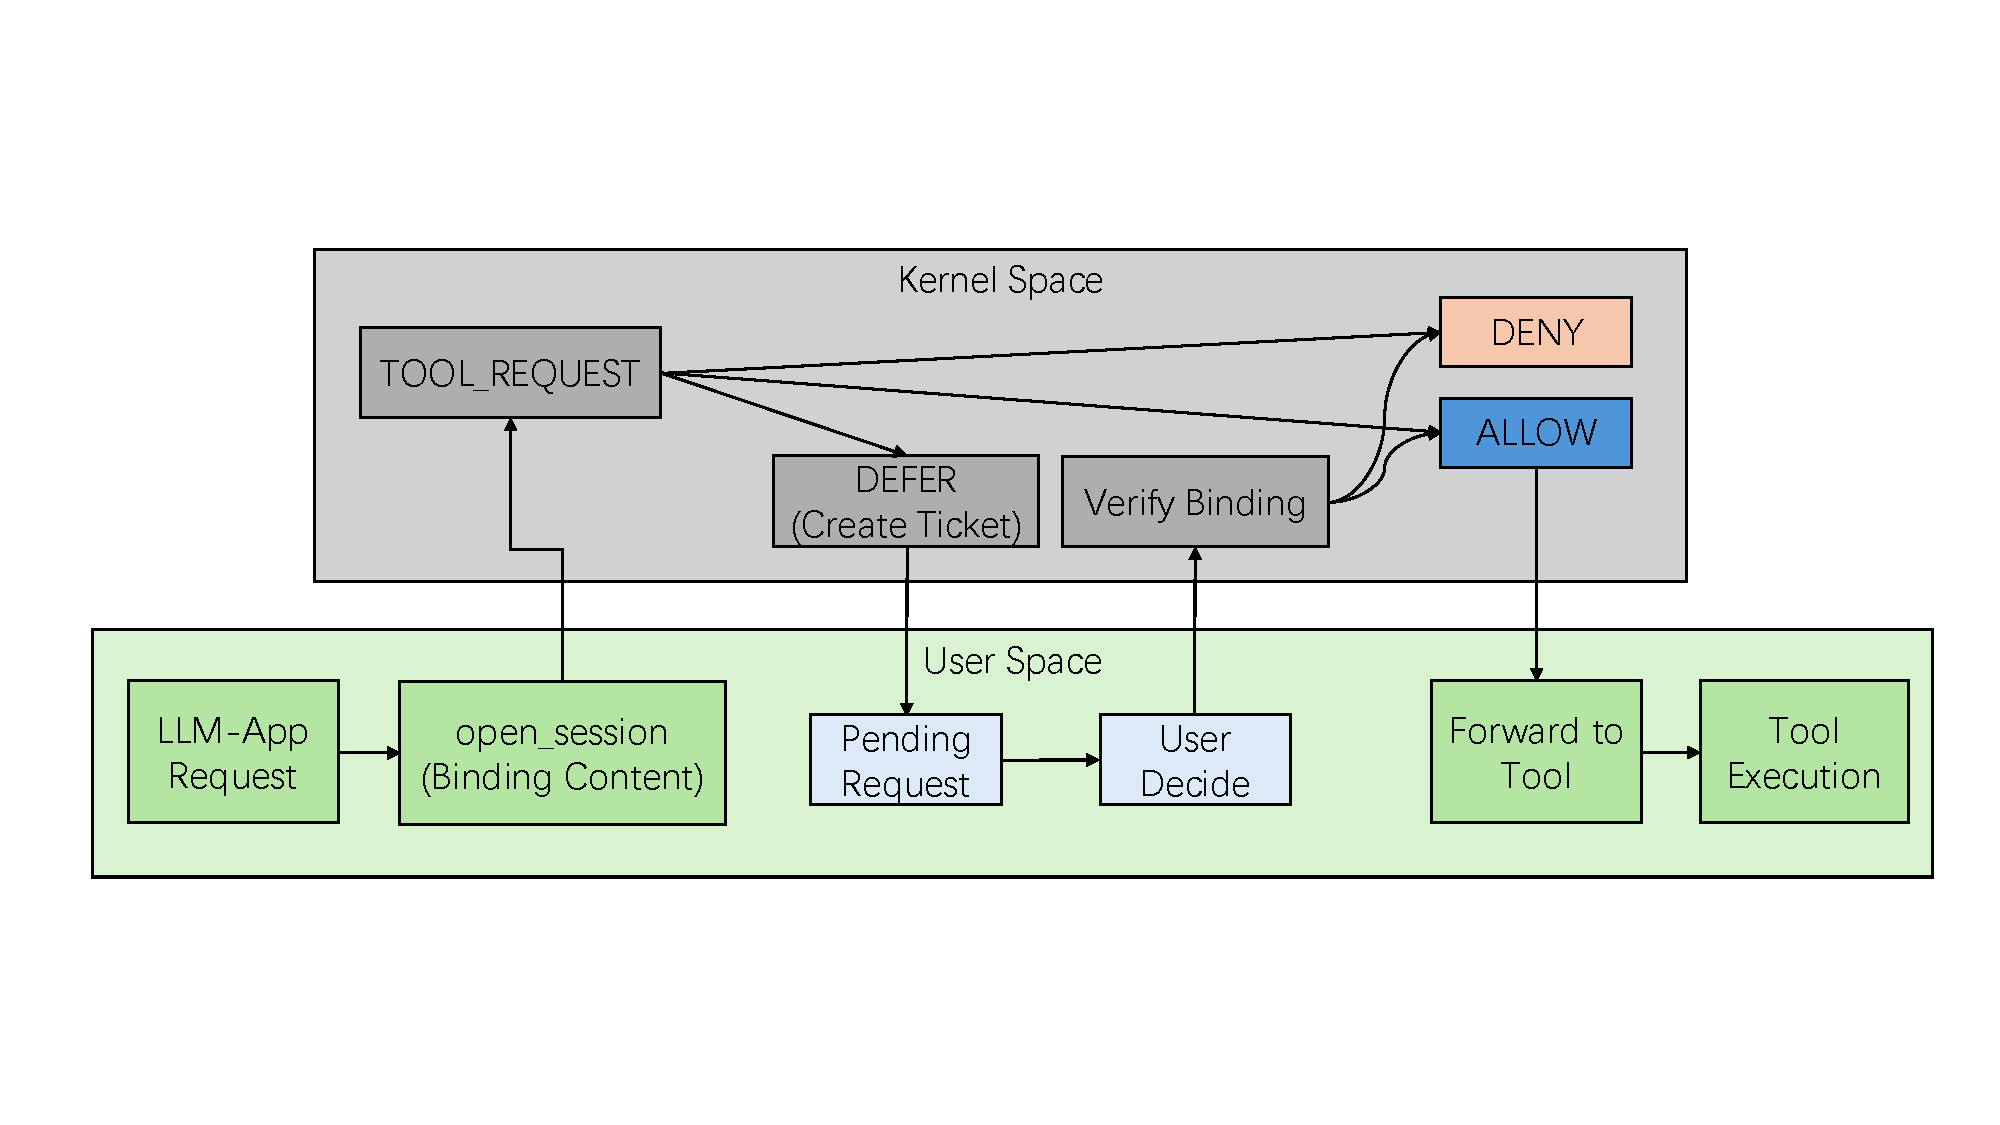
\includegraphics[width=\linewidth,trim=0.5cm 2cm 0cm 2cm,clip]{figures/linux-mcp-approval.pdf}
\caption{Approval-ticket flow in \texttt{linux-mcp}: the \texttt{ALLOW}/\texttt{DENY}/\texttt{DEFER} state machine enforced by the kernel module.}
\label{fig:chapter3-approval}
\end{figure}



\subsection{Kernel Module Design}

\texttt{kernel\_\allowbreak mcp} is implemented as a loadable kernel module exposing the \texttt{KERNEL\_\allowbreak MCP} Generic Netlink family.
The command set covers the full invocation lifecycle: \texttt{TOOL\_\allowbreak REGISTER}, \texttt{AGENT\_\allowbreak REGISTER}, \texttt{TOOL\_\allowbreak REQUEST}, \texttt{TOOL\_\allowbreak DECISION}, \texttt{TOOL\_\allowbreak COMPLETE}, \texttt{APPROVAL\_\allowbreak DECIDE}, \texttt{RESET\_\allowbreak TOOLS}, and \texttt{LIST\_\allowbreak TOOLS}.
Generic Netlink was chosen over \texttt{ioctl} or character devices because it provides structured messages, supports dump-style enumeration for registry introspection, and is well suited to a research prototype~\cite{netlink2026}.

Internally, the module maintains two registries.
The tool registry maps tool identifiers to their manifest-derived semantic hashes and associated metadata.
The agent registry records the identifiers of entities permitted to submit requests through the control plane.
Approval tickets are heap-allocated kernel objects with explicit lifecycle fields tracking whether a ticket has been decided, approved, consumed, or expired.

The arbitration logic is deliberately narrow.
For a \texttt{TOOL\_\allowbreak REQUEST} to be admitted, three conditions must all hold: the submitting agent must appear in the agent registry, the target tool must appear in the tool registry, and the semantic hash supplied by \texttt{mcpd} must match the hash recorded at registration time.
If the tool's manifest marks it as requiring explicit approval, the request is deferred rather than immediately allowed.

\paragraph{Trust-on-first-use backend binary pinning.}
Semantic-hash admission guards what a tool claims to be, not which binary actually serves the socket.
The kernel therefore keeps a per-tool \texttt{binary\_\allowbreak hash} slot populated on first use: \texttt{mcpd} reads the backend's peer PID via \texttt{SO\_\allowbreak PEERCRED} and hashes \texttt{/\allowbreak proc/\allowbreak <pid>/\allowbreak exe}, using a composite digest over interpreter plus script for interpreter-hosted tools so a script swap is still caught.
The digest is attached to the first \texttt{TOOL\_\allowbreak REGISTER}; later registrations or requests carrying a different digest are rejected.
A \texttt{binary\_\allowbreak hash\_\allowbreak state} field (\texttt{unpinned} or \texttt{live\_\allowbreak pinned}) distinguishes ``no probe yet'' from ``pinned'', since both previously read as an empty string.

\paragraph{Kernel-resident call log.}
Each agent carries a fixed-size circular buffer of invocation records.
A record is a flat struct: request id, timestamp, tool id, status, execution latency, a tool status code (analogous to a process exit code), 8-byte payload and response hash prefixes, and the leading bytes of any error output.
Records are written on both the \texttt{ALLOW}+\texttt{TOOL\_\allowbreak COMPLETE} and \texttt{DENY}/\texttt{DEFER} paths, so successful, rejected, and deferred invocations are all captured.
The kernel does no JSON parsing; \texttt{mcpd} precomputes the hashes and passes them as fixed-width attributes.
The buffer is exported through \texttt{sysfs} as a binary attribute, so recent history can be read back after \texttt{mcpd} crashes.
This is crash-visible audit, not tamper-evident provenance: the buffer is bounded and the hashes are 8-byte prefixes.

\paragraph{Sysfs surface.}
Under \texttt{/\allowbreak sys/\allowbreak kernel/\allowbreak mcp/\allowbreak tools/}, each tool directory exposes \texttt{name}, semantic \texttt{hash}, \texttt{binary\_\allowbreak hash}, \texttt{binary\_\allowbreak hash\_\allowbreak state}, and \texttt{registered\_\allowbreak at\_\allowbreak epoch}; the global \texttt{tool\_\allowbreak catalog\_\allowbreak epoch} sits at the top of the tree.
Under \texttt{/\allowbreak sys/\allowbreak kernel/\allowbreak mcp/\allowbreak agents/}, per-agent entries expose \texttt{allow}/\texttt{defer}/\texttt{completed\_\allowbreak ok}/\texttt{last\_\allowbreak exec\_\allowbreak ms} counters, a human-readable \texttt{last\_\allowbreak reason}, and the \texttt{call\_log} above with its head and count indices.
This lets an operator check what the kernel regards as authoritative without relying on daemon-side logs.



\subsection{Daemon Implementation}
\label{sec:daemon-implementation}

The kernel enforces the critical state transitions, but \texttt{mcpd} does most of the actual work.
It is organised around four modules: manifest loading and semantic hashing, session storage and binding-context management, Netlink communication with the kernel, and request forwarding to tool services.

The manifest loader is the semantic entry point of the system, producing both the kernel registry entries and the catalog served to \texttt{llm-app} in response to \texttt{list\_apps} and \texttt{list\_\allowbreak tools} queries.

The session store maintains active connections together with their peer-derived binding information and any pending approval context.
This gives the daemon sufficient information to associate incoming approval decisions with the correct deferred request, without requiring the kernel to store full session semantics.
The binding information, derived from Unix domain socket peer credentials, is what gets embedded in approval tickets.

The Netlink client provides a persistent communication channel to the kernel module.
A dedicated, long-lived socket is maintained rather than opening a new connection per request; this keeps the control path measurable and avoids repeated socket-setup overhead.
Per-stage timing covering session lookup, kernel arbitration, tool execution, and end-to-end latency can optionally be recorded for each invocation, which is useful for separating control-plane overhead from tool-side processing time during evaluation.

The server-facing side of \texttt{mcpd} handles two distinct roles: it exposes the catalog and invocation interfaces consumed by \texttt{llm-app}, and it forwards admitted requests to the appropriate \texttt{tool-app} service via the same Unix domain socket transport used on the tool side.

\paragraph{Deployment and fail-closed configuration.}
\texttt{mcpd} needs \texttt{CAP\_\allowbreak NET\_\allowbreak ADMIN} for Netlink administration and \texttt{CAP\_\allowbreak SYS\_\allowbreak PTRACE} for reading \texttt{/\allowbreak proc/\allowbreak <pid>/\allowbreak exe} across uid boundaries during the backend probe.
The supplied systemd unit grants both via \texttt{Ambient\allowbreak Capabilities} and runs the daemon as an unprivileged \texttt{mcpd} user with \texttt{No\allowbreak New\allowbreak Privileges} and a read-only bind mount of the manifest directory, so gateway RCE cannot load kernel modules or mutate manifests.

A separate question is which UIDs the daemon accepts as tool backends.
\texttt{allowed\_\allowbreak backend\_\allowbreak uids} is checked via \texttt{SO\_\allowbreak PEERCRED} on both probe and exec dials.
An unprivileged \texttt{mcpd} defaults to its own UID.
A privileged \texttt{mcpd} has no safe default: trusting only UID~0 would reject every realistic non-root backend and leave \texttt{binary\_\allowbreak hash} unpinned, while trusting \texttt{\$SUDO\_\allowbreak UID} would fold launcher-script state into the daemon's trust boundary.
The daemon therefore refuses to start unless the list is declared in the TOML or the operator explicitly opts in to \texttt{\$SUDO\_\allowbreak UID} trust via an environment variable.



\subsection{Tool-Side RPC and Execution Model}

The tool-side protocol (detailed in Table~\ref{tab:mcpd-toolapp}) is intentionally minimal: each tool service is a resident process bound to a Unix domain socket with no kernel-facing obligations.
Because the boundary between admission and execution is drawn at the kernel, the boundary within user space is equally unambiguous: the kernel decides whether a request may proceed; everything concerning what the request means and how it is executed remains in user space.
Failure handling follows naturally from this separation.
If a tool crashes, times out, or returns an error, \texttt{mcpd} handles the event in user space and reflects it back to the kernel through \texttt{TOOL\_\allowbreak COMPLETE}, marking the invocation lifecycle as closed.
The kernel requires no visibility into how the tool failed internally.



\subsection{State Reconciliation and Recovery}
\label{sec:reconciliation}

\texttt{linux-mcp} treats daemon restart as a recovery problem rather than a process-management detail. The kernel remains authoritative for the tool registry, approval tickets, the global \texttt{tool\_\allowbreak catalog\_\allowbreak epoch}, and the per-agent \texttt{call\_log}; the manifest set on disk remains the source of truth for tool identity. By contrast, open sessions, peer-credential bindings, and pending request maps live only in \texttt{mcpd} and are discarded on restart.

Recovery is therefore conservative. At cold start, \texttt{mcpd} issues \texttt{RESET\_\allowbreak TOOLS} and re-registers the current manifest set unconditionally. During normal operation, reconciliation is incremental: only tools whose \texttt{manifest\_\allowbreak hash} or \texttt{binding\_\allowbreak fingerprint} changed are re-registered, and each such update advances both the tool's \texttt{registered\_\allowbreak at\_\allowbreak epoch} and the global epoch. If the backend's peer UID or resolved binary digest changes, the kernel TOFU slot is cleared before re-registration so the new identity is pinned afresh rather than inherited from the old one.

This split preserves audit and admission state without pretending that a crashed daemon can safely continue old sessions. Approval tickets and registry history remain inspectable through \texttt{sysfs}, but clients must reopen any session that pre-dates the restart before issuing a new \texttt{TOOL\_\allowbreak REQUEST}. A kernel module reload remains outside the recovery model and is treated as a fresh system.



\subsection{Rationale for the Kernel--User-Space Split}
\label{sec:design-alternatives}

Three kernel-interface designs were tried or seriously considered before settling on Generic Netlink.

The first attempt used eBPF.
It seemed like a natural fit: lightweight, no full kernel module needed, and increasingly the standard approach for extending kernel behaviour.
The problem appeared once the approval-ticket lifecycle had to be implemented: a ticket is created on \texttt{DEFER}, updated on \texttt{APPROVAL\_\allowbreak DECIDE}, consumed on the second \texttt{TOOL\_\allowbreak REQUEST}, and eventually expired.
That is inherently stateful across multiple messages, and the eBPF verifier's restrictions on loops and on persistent mutable state made it impractical to express.
Keeping the ticket state in a user-space map would have reintroduced exactly the durability problem the kernel placement was meant to solve.

LSM hooks were the second candidate.
They fire at the syscall boundary, which is the wrong layer: tool identity in this system is a SHA-256 hash of a JSON manifest, not a file path or a socket operation.
There is no syscall at which the kernel naturally sees a tool hash alongside a request; correlating the two would require injecting application-layer semantics into a mechanism designed for OS-object-level policy.
The mismatch was fundamental, not a matter of implementation effort.

A capability-based design (in the style of Capsicum) was also considered.
It would have required tool services to interact with a kernel-facing API to obtain and present capabilities, breaking the goal that tool authors need only write a JSON manifest with no kernel-facing obligations.

Generic Netlink avoids all three problems.
It supports structured TLV messages, dump-style enumeration for registry introspection, and arbitrary internal state management in a loadable module.
The cost is that a full kernel module is needed, where a policy hook or a BPF program would have sufficed for simpler designs. For a research prototype this is an acceptable trade-off, and in practice the module's role stayed narrow enough that the added complexity remained manageable.



\subsection{Limitations and Identified Optimisation Opportunities}

The prototype makes several deliberate simplifications.
A single global lock protects the kernel registries; this is adequate at evaluated catalog sizes but a scalability concern under higher concurrency.
Cold-start reconciliation is unconditional: every launch pays a \texttt{RESET\_\allowbreak TOOLS} plus a full \texttt{TOOL\_\allowbreak REGISTER} sweep, even when manifests are unchanged.
Hot reload is request-driven rather than filesystem-driven: \texttt{mcpd} recomputes a manifest-set signature on the \texttt{list\_apps}, \texttt{list\_\allowbreak tools}, and \texttt{tool:exec} paths and refreshes the kernel registry when the signature changes, so a manifest edit takes effect on the next request rather than the instant the file is written.
The kernel does no per-agent rate limiting; throttling is left to \texttt{mcpd}.
Resolution directions are discussed in Section~\ref{sec:further-work}.
